% Original Author: GitHub @leowrs (https://github.com/leowrs)
\documentclass[12pt]{article}
\usepackage{amsmath}
\usepackage{amsfonts}
\usepackage{tikz}
\usepackage{tikz-qtree}
\usepackage{fancyhdr}  % 用于设置页眉页脚
\usepackage{tipa}      % 添加IPA语音符号支持

% 使用fontspec和xeCJK来设置字体
\usepackage{fontspec}
\usepackage{xeCJK}
\setmainfont{Times New Roman}  % 设置英文字体为Times New Roman
\setCJKmainfont{SimSun}  % 设置中文字体为宋体
\setCJKmonofont{SimSun}  % 设置中文等宽字体，修复CJKttdefault警告

% 设置页眉高度
\setlength{\headheight}{15pt}  % 修复headheight警告

% 设置页眉
\pagestyle{fancy}
\fancyhf{}  % 清除所有页眉页脚
\fancyhead[L]{HW1.2: Morphology}
\fancyhead[C]{@leowrs}
\fancyhead[R]{—}
\renewcommand{\headrulewidth}{0.4pt}  % 页眉横线

\begin{document}

% 确保第一页也有页眉
\thispagestyle{fancy}

\section*{HW1.2: Morphology}

\subsection*{I.}

\noindent \textbf{(1) disappearance}

\noindent \textbf{Tree Diagram:}
\begin{tikzpicture}[level distance=1.5cm, 
                    level 1/.style={sibling distance=3cm},
                    level 2/.style={sibling distance=2cm},
                    level 3/.style={sibling distance=1.5cm}]
\node {Noun}
    child {node {dis-}
    }
    child {node {Noun}
            child {node {Verb}
                child {node {appear}}
            }
            child {node {-ance}
            }
    };
\end{tikzpicture}

\noindent \textbf{Morphological Rules:}
\begin{enumerate}
    \item \texttt{appear + -ance $\rightarrow$ appearance} (Verb + Nominalizing suffix)
    \item \texttt{dis- + appearance $\rightarrow$ disappearance} (Negative prefix + Noun)
\end{enumerate}

\bigskip

\noindent \textbf{(2) irreplaceability}

\noindent \textbf{Tree Diagram:}
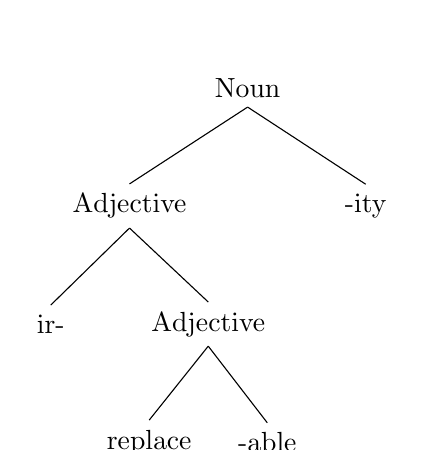
\begin{tikzpicture}[level distance=1.5cm, 
                    level 1/.style={sibling distance=3cm},
                    level 2/.style={sibling distance=2cm},
                    level 3/.style={sibling distance=1.5cm}]
\node {Noun}
    child {node {Adjective}
        child {node {ir-}
        }
        child {node {Adjective}
            child {node {replace}}
            child {node {-able}}
        }
    }
    child {node {-ity}
    };
\end{tikzpicture}

\noindent \textbf{Morphological Rules:}
\begin{enumerate}
    \item \texttt{replace + -able $\rightarrow$ replaceable} (Verb + Adjectival suffix)
    \item \texttt{replaceable + -ity $\rightarrow$ replaceability} (Adjective + Nominalizing suffix)
\end{enumerate}

\bigskip

\noindent \textbf{(3) misconceive}

\noindent \textbf{Tree Diagram:}
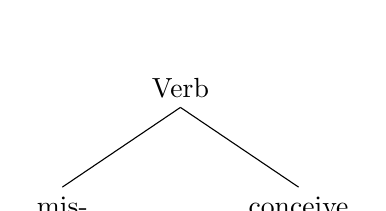
\begin{tikzpicture}[level distance=1.5cm, 
                    level 1/.style={sibling distance=3cm}]
\node {Verb}
    child {node {mis-}
    }
    child {node {conceive}
    };
\end{tikzpicture}

\noindent \textbf{Morphological Rules:}
\begin{enumerate}
    \item \texttt{mis- + conceive $\rightarrow$ misconceive} (Negative Prefix + Verb)
\end{enumerate}

\bigskip

\subsection*{II.}

\noindent \textbf{(a) 'able to be less dark'}

\noindent \textbf{Tree Diagram:}
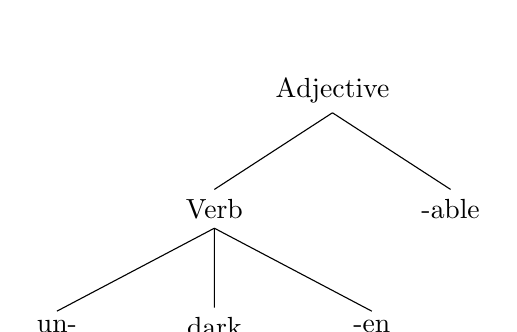
\begin{tikzpicture}[level distance=1.5cm, 
                    level 1/.style={sibling distance=3cm},
                    level 2/.style={sibling distance=2cm}]
\node {Adjective}
    child {node {Verb}
        child {node {un-}}
        child {node {dark}}
        child {node {-en}}
    }
    child {node {-able}
    };
\end{tikzpicture}
\bigskip

\noindent \textbf{(b) 'unable to be made dark'}

\noindent \textbf{Tree Diagram:}
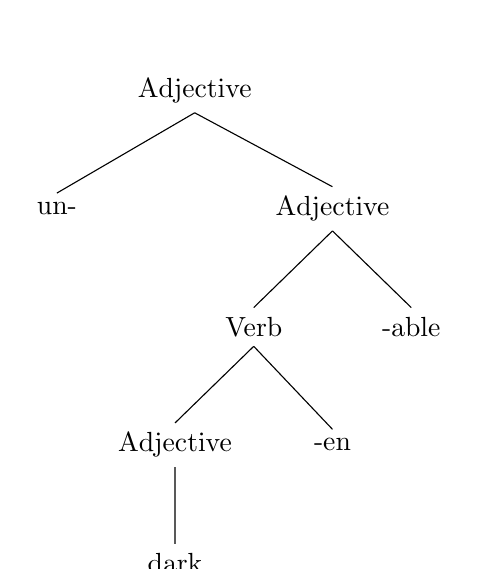
\begin{tikzpicture}[level distance=1.5cm, 
                    level 1/.style={sibling distance=3.5cm},
                    level 2/.style={sibling distance=2cm}]
\node {Adjective}
    child {node {un-}
    }
    child {node {Adjective}
        child {node {Verb}
                child {node {Adjective}
                child {node {dark}}
            }
            child {node {-en}}
        } 
        child {node {-able}
        } 
    };
\end{tikzpicture}

\subsection*{III.}

\noindent \textbf{(1) defamiliarized (past tense)}

\noindent \textbf{Tree Diagram:}
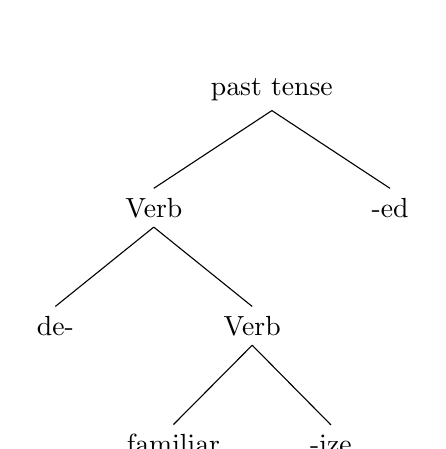
\begin{tikzpicture}[level distance=1.5cm, 
                    level 1/.style={sibling distance=3cm},
                    level 2/.style={sibling distance=2.5cm},
                    level 3/.style={sibling distance=2cm}]
\node {past tense}
    child {node {Verb}
        child {node {de-}
        }
        child {node {Verb}
            child {node {familiar}}
            child {node {-ize}}
        }
    }
    child {node {-ed}
    };
\end{tikzpicture}

\bigskip

\noindent \textbf{(2) unlikeliest (superlative)}

\noindent \textbf{Tree Diagram:}
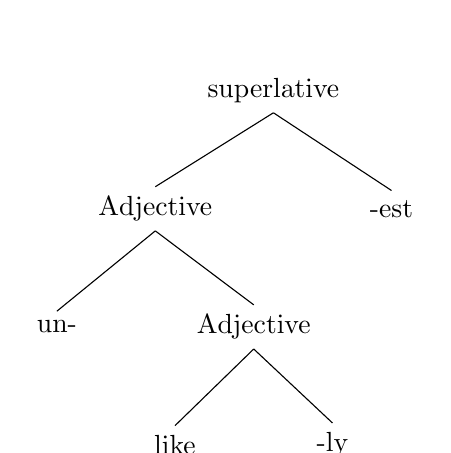
\begin{tikzpicture}[level distance=1.5cm, 
                    level 1/.style={sibling distance=3cm},
                    level 2/.style={sibling distance=2.5cm},
                    level 3/.style={sibling distance=2cm}]
\node {superlative}
    child {node {Adjective}
        child {node {un-}}
        child {node {Adjective}
            child {node {like}}
            child {node {-ly}}
        }
    }
    child {node {-est}
    };
\end{tikzpicture}

\section*{IV. Sanskrit}

\noindent \textbf{(1) Sanskrit morphemes:}

\begin{itemize}
    \item gen.sg.  $\rightarrow$ \texttt{-as}
    \item dat.sg.  $\rightarrow$ \texttt{-e}
    \item inst.sg. $\rightarrow$ \texttt{-ā}
    \item gen.pl.  $\rightarrow$ \texttt{-ām}
    \item dat.pl.  $\rightarrow$ \texttt{-bhyas}
    \item loc.sg.  $\rightarrow$ \texttt{-i}
\end{itemize}

\bigskip

\noindent \textbf{(2) Allomorphs:}

\begin{itemize}
    \item 'mind': \texttt{mano}
    \item 'wonder': \texttt{vapuʂ, vapur}
    \item 'devout': \texttt{suhaviʂ, suhavir}
\end{itemize}

\bigskip

\noindent \textbf{(3) Conditioning environment:}

\begin{enumerate}[label=\arabic*., leftmargin=*]
  \item \textbf{Stems ending in a high vowel (e.g., \textit{i}):}
  \begin{itemize}[label=--]
      \item When adding a \textbf{vowel-initial suffix}, the final \textit{s} becomes retroflex \textit{ʂ} (e.g., \textit{asti} → \textit{aʂ + i}).
      \item When adding a \textbf{consonant-initial suffix}, a high vowel requires insertion of \textit{r} and the final \textit{s} drops (e.g., \textit{i + consonant} → \textit{ir + consonant}).
  \end{itemize}
  
  \item \textbf{Stems ending in a central/low vowel (e.g., \textit{a}):}
  
\begin{itemize}[label=--]
      \item When adding a \textbf{vowel-initial suffix}, the final \textit{s} remains unchanged (e.g., \textit{dasa + a} → \textit{dasa + a}).
      \item When adding a \textbf{consonant-initial suffix}, the low vowel undergoes sandhi (phonetic fusion), and the final \textit{s} drops (e.g., \textit{a + consonant} → fused vowel variant).
  \end{itemize}
\end{enumerate}

\textbf{Universal Rule}: Regardless of the stem’s vowel type, the final \textit{s} is \textbf{always deleted} before consonant-initial suffixes. These rules ensure syllabic harmony and phonetic fluency in compound forms.


\end{document}
